% appendix/questions/questions.tex
% SPDX-License-Identifier: CC-BY-SA-3.0

\QuickQuizChapter{cha:app:Important Questions}{Important Questions}

\epigraph{Ask me no questions, and I'll tell you no fibs.}
	 {\emph{``She Stoops to Conquer'', Oliver Goldsmith}}

The following sections discuss some important questions relating to
SMP programming.
Each section also shows how to {\em avoid} having to worry about
the corresponding question, which can be extremely important if
your goal is to simply get your SMP code working as quickly and
painlessly as possible---which is an excellent goal, by the way!

Although the answers to these questions are often quite a bit less
intuitive than they would be in a single-threaded setting,
with a bit of work, they are not that difficult to understand.
If you managed to master recursion, there is nothing in here that should
pose an overwhelming challenge.

% @@@ roadmap...

% @@@ doesn't parallel automatically make things faster? (locked increment)
% @@@ doesn't getting rid of locks get rid of all these problems? (atomic inc)
% @@@ doesn't NBS take care of all these problems? (cite IPDPS paper)

% appendix/questions/after.tex

\section{What Does ``After'' Mean?}
\label{sec:app:questions:What Does ``After'' Mean?}

``After'' 는 직관적이지만 놀라우리만큼 어려운 개념입니다.
한가지 중요한 반직관적 문제는 코드가 언제든 얼만큼이든 지연되어서 수행될 수
있다는 점입니다.
타임스탬프 ``t'' 와 정수 필드 ``a'', ``b'', 그리고 ``c'' 를 포함하는 글로벌
구조체를 이용해서 통신을 하는 생산자와 소비자 구조를 생각해 봅시다.
생산자는
Figure~\ref{fig:app:questions:After Producer Function} 에 보여진 것처럼
(1970 년으로부터의 현재 시각까지 지난 초를 10진수로 나타내는) 현재 시각을
기록하고 ``a'', ``b'', 그리고 ``c'' 를 업데이트 하는 루프를 돕니다.
소비자는
Figure~\ref{fig:app:questions:After Consumer Function} 에 보여진 것처럼 역시
현재 시각을 기록하지만 생성자의 타임스탬프와 ``a'', ``b'', 그리고 ``c'' 필드의
값을 복사해 옵니다.
프로그램 수행 종료 시점에서, 소비자는 이례적인 기록들을 출력하는데, 예를 들면
시간이 뒤로 돌아간 것으로 보이는 경우입니다.
\iffalse

``After'' is an intuitive, but surprisingly difficult concept.
An important non-intuitive issue is that code can be delayed at
any point for any amount of time.
Consider a producing and a consuming thread that communicate using
a global struct with a timestamp ``t'' and integer fields ``a'', ``b'',
and ``c''.
The producer loops recording the current time
(in seconds since 1970 in decimal),
then updating the values of ``a'', ``b'', and ``c'',
as shown in Figure~\ref{fig:app:questions:After Producer Function}.
The consumer code loops, also recording the current time, but also
copying the producer's timestamp along with the fields ``a'',
``b'', and ``c'', as shown in
Figure~\ref{fig:app:questions:After Consumer Function}.
At the end of the run, the consumer outputs a list of anomalous recordings,
e.g., where time has appeared to go backwards.
\fi

\begin{figure}[htbp]
{ \scriptsize
\begin{verbbox}
  1 /* WARNING: BUGGY CODE. */
  2 void *producer(void *ignored)
  3 {
  4   int i = 0;
  5
  6   producer_ready = 1;
  7   while (!goflag)
  8     sched_yield();
  9   while (goflag) {
 10     ss.t = dgettimeofday();
 11     ss.a = ss.c + 1;
 12     ss.b = ss.a + 1;
 13     ss.c = ss.b + 1;
 14     i++;
 15   }
 16   printf("producer exiting: %d samples\n", i);
 17   producer_done = 1;
 18   return (NULL);
 19 }
\end{verbbox}
}
\centering
\theverbbox
\caption{``After'' Producer Function}
\label{fig:app:questions:After Producer Function}
\end{figure}

\begin{figure}[htbp]
{ \scriptsize
\begin{verbbox}
  1 /* WARNING: BUGGY CODE. */
  2 void *consumer(void *ignored)
  3 {
  4   struct snapshot_consumer curssc;
  5   int i = 0;
  6   int j = 0;
  7
  8   consumer_ready = 1;
  9   while (ss.t == 0.0) {
 10     sched_yield();
 11   }
 12   while (goflag) {
 13     curssc.tc = dgettimeofday();
 14     curssc.t = ss.t;
 15     curssc.a = ss.a;
 16     curssc.b = ss.b;
 17     curssc.c = ss.c;
 18     curssc.sequence = curseq;
 19     curssc.iserror = 0;
 20     if ((curssc.t > curssc.tc) ||
 21         modgreater(ssc[i].a, curssc.a) ||
 22         modgreater(ssc[i].b, curssc.b) ||
 23         modgreater(ssc[i].c, curssc.c) ||
 24         modgreater(curssc.a, ssc[i].a + maxdelta) ||
 25         modgreater(curssc.b, ssc[i].b + maxdelta) ||
 26         modgreater(curssc.c, ssc[i].c + maxdelta)) {
 27       i++;
 28       curssc.iserror = 1;
 29     } else if (ssc[i].iserror)
 30       i++;
 31     ssc[i] = curssc;
 32     curseq++;
 33     if (i + 1 >= NSNAPS)
 34       break;
 35   }
 36   printf("consumer exited, collected %d items of %d\n",
 37          i, curseq);
 38   if (ssc[0].iserror)
 39     printf("0/%d: %.6f %.6f (%.3f) %d %d %d\n",
 40            ssc[0].sequence, ssc[j].t, ssc[j].tc,
 41            (ssc[j].tc - ssc[j].t) * 1000000,
 42            ssc[j].a, ssc[j].b, ssc[j].c);
 43   for (j = 0; j <= i; j++)
 44     if (ssc[j].iserror)
 45       printf("%d: %.6f (%.3f) %d %d %d\n",
 46              ssc[j].sequence,
 47              ssc[j].t, (ssc[j].tc - ssc[j].t) * 1000000,
 48              ssc[j].a - ssc[j - 1].a,
 49              ssc[j].b - ssc[j - 1].b,
 50              ssc[j].c - ssc[j - 1].c);
 51   consumer_done = 1;
 52 }
\end{verbbox}
}
\centering
\theverbbox
\caption{``After'' Consumer Function}
\label{fig:app:questions:After Consumer Function}
\end{figure}

\QuickQuiz{}
	이 예제에서 어떤 SMP 코딩 에러가 보이나요?
	전체 코드를 보기 위해선 \path{time.c} 파일을 보세요.
	\iffalse

	What SMP coding errors can you see in these examples?
	See \path{time.c} for full code.
	\fi
\QuickQuizAnswer{
	\begin{enumerate}
	\item	루프에서 barrier() 나 volatile 을 사용하지 않음.
	\item	업데이트 쪽에서 메모리 배리어를 사용하지 않음.
	\item	생성자와 소비자 사이의 동기화가 없음.
	\iffalse

	\item	Missing barrier() or volatile on tight loops.
	\item	Missing Memory barriers on update side.
	\item	Lack of synchronization between producer and consumer.
	\fi
	\end{enumerate}
} \QuickQuizEnd

생성자가 타임스탬프나 값들을 저장하는데에 그렇게 많은 시간이 걸리지 않을
것이기에 생성자와 소비자 타임스탬프 간의 차이는 상당히 작을 것이라고 예상하는
사람들이 있겠습니다.
듀얼코어 1GHz x86 에서의 출력 결과가
Table~\ref{tab:app:questions:After Program Sample Output} 에 보여져 있습니다.
여기서, ``seq'' 행은 루프를 수행한 횟수이고, ``time'' 행은 변칙적 행위가 나타난
시각을 초로 나타낸 것이고, ``delta'' 행은 소비자의 타임스탬프가 생성자의 것보다
얼마나 뒤의 것이었는지 (즉, 이 값이 음수라면 소비자가 생성자보다 타임스탬프를
먼저 받았음을 말합니다), 그리고 ``a'', ``b'', 그리고 ``c'' 로 나타내어진 행들은
이 변수들이 소비자에 의해 수집된 앞의 스냅샷에 비해 얼마나 증가되었는지를
보입니다.
\iffalse

One might intuitively expect that the difference between the producer
and consumer timestamps would be quite small, as it should not take
much time for the producer to record the timestamps or the values.
An excerpt of some sample output on a dual-core 1GHz x86 is shown in
Table~\ref{tab:app:questions:After Program Sample Output}.
Here, the ``seq'' column is the number of times through the loop,
the ``time'' column is the time of the anomaly in seconds, the ``delta''
column is the number of seconds the consumer's timestamp follows that
of the producer (where a negative value indicates that the consumer
has collected its timestamp before the producer did), and the
columns labelled ``a'', ``b'', and ``c'' show the amount that these
variables increased since the prior snapshot collected by the consumer.
\fi

\begin{table}[htbp]
\centering
\scriptsize
\begin{tabular}{rcrrrr}
seq    & time (seconds) & delta~    &  a &  b &  c \\
\hline
17563: & 1152396.251585 & ($-16.928$) & 27 & 27 & 27 \\
18004: & 1152396.252581 & ($-12.875$) & 24 & 24 & 24 \\
18163: & 1152396.252955 & ($-19.073$) & 18 & 18 & 18 \\
18765: & 1152396.254449 & ($-148.773$) & 216 & 216 & 216 \\
19863: & 1152396.256960 & ($-6.914$) & 18 & 18 & 18 \\
21644: & 1152396.260959 & ($-5.960$) & 18 & 18 & 18 \\
23408: & 1152396.264957 & ($-20.027$) & 15 & 15 & 15 \\
\end{tabular}
\caption{``After'' Program Sample Output}
\label{tab:app:questions:After Program Sample Output}
\end{table}

왜 시간이 거꾸로 가는 걸까요?
괄호 안의 숫자는 마이크로세컨드 단위의 차이로써, 큰 수는 10 마이크로세컨드를
넘기고, 한번은 100 마이크로세컨드를 넘기기조차 했습니다!
이 CPU 는 그동안 100,000 개의 인스트럭션을 수행할 수도 있음을 알아두시기
바랍니다.

한가지 가능한 이유는 다음과 같은 이벤트 시퀀스로 설명됩니다:
\iffalse

Why is time going backwards?
The number in parentheses is the difference in microseconds, with
a large number exceeding 10 microseconds, and one exceeding even
100 microseconds!
Please note that this CPU can potentially execute more than 100,000
instructions in that time.

One possible reason is given by the following sequence of events:
\fi
\begin{enumerate}
\item	소비자가 타임스탬프를 얻어옵니다
	(Figure~\ref{fig:app:questions:After Consumer Function}, line~13).
\item	소비자가 preemption 당합니다.
\item	임의의 시간이 흐릅니다.
\item	생성자가 타임스탬프를 얻어옵니다
	(Figure~\ref{fig:app:questions:After Producer Function}, line~10).
\item	소비자가 수행을 다시 재개하고, 생성자의 타임스탬프를 읽어옵니다
	(Figure~\ref{fig:app:questions:After Consumer Function}, line~14).
\iffalse

\item	Consumer obtains timestamp
	(Figure~\ref{fig:app:questions:After Consumer Function}, line~13).
\item	Consumer is preempted.
\item	An arbitrary amount of time passes.
\item	Producer obtains timestamp
	(Figure~\ref{fig:app:questions:After Producer Function}, line~10).
\item	Consumer starts running again, and picks up the producer's
	timestamp
	(Figure~\ref{fig:app:questions:After Consumer Function}, line~14).
\fi
\end{enumerate}

이 시나리오 상에서, 생성자의 타임스탬프는 소비자의 타임스탬프보다 얼만큼이든
뒤의 것일 수 있습니다.

여러분은 여러분의 SMP 코드가 ``after'' 의 의미로 고민하는 것을 어떻게
막으시나요?

그냥 SMP 기능들을 설계된 대로 사용하세요.
\iffalse

In this scenario, the producer's timestamp might be an arbitrary
amount of time after the consumer's timestamp.

How do you avoid agonizing over the meaning of ``after'' in your
SMP code?

Simply use SMP primitives as designed.
\fi

이 예제에서, 가장 간단한 수정방법은 락킹을 사용하는 것으로, 예를 들어 생성자는
Figure~\ref{fig:app:questions:After Producer Function} 의 line~10 앞에서 락을
잡고 소비자는
Figure~\ref{fig:app:questions:After Consumer Function} 의 line~13 앞에서 락을
잡도록 합니다.
또한, 이 락은
Figure~\ref{fig:app:questions:After Producer Function} 의 line~13 뒤에서
해제되고
Figure~\ref{fig:app:questions:After Consumer Function} 의 line~17 뒤에서
해제되어야만 합니다.
이 락들은
Figure~\ref{fig:app:questions:After Producer Function} 의 line~10-13 과
Figure~\ref{fig:app:questions:After Consumer Function} 의 line~13-17 의 코드
조각들이 서로를 {\em 배제} 하도록 해주는데, 달리 말하자면 서로에 대해서
어토믹하게 수행되게 된다는 말입니다.
이는
Figure~\ref{fig:app:questions:Effect of Locking on Snapshot Collection} 로
표현되어 있습니다:
이 락킹은 모든 상자 안의 코드가 시간상으로 겹쳐지는 것을 방지해 줘서, 소비자의
타임스탬프는 앞의 생성자의 타임스탬프 뒤에 수집될 수 있도록 해줍니다.
이 그림에 있는 각각의 상자 안의 코드 조각들은 ``크리티컬 섹션'' 이라
명명됩니다; 한 시점에는 오로지 하나의 크리티컬 섹션만이 수행됩니다.
\iffalse

In this example, the easiest fix is to use locking, for example,
acquire a lock in the producer before line~10 in
Figure~\ref{fig:app:questions:After Producer Function} and in
the consumer before line~13 in
Figure~\ref{fig:app:questions:After Consumer Function}.
This lock must also be released after line~13 in
Figure~\ref{fig:app:questions:After Producer Function} and
after line~17 in
Figure~\ref{fig:app:questions:After Consumer Function}.
These locks cause the code segments in lines~10-13 of
Figure~\ref{fig:app:questions:After Producer Function} and in lines~13-17 of
Figure~\ref{fig:app:questions:After Consumer Function} to {\em exclude}
each other, in other words, to run atomically with respect to each other.
This is represented in
Figure~\ref{fig:app:questions:Effect of Locking on Snapshot Collection}:
the locking prevents any of the boxes of code from overlapping in time, so
that the consumer's timestamp must be collected after the prior
producer's timestamp.
The segments of code in each box in this figure are termed
``critical sections''; only one such critical section may be executing
at a given time.
\fi

\begin{figure}[htb]
\centering
\includegraphics{appendix/questions/after-snapshot}
\caption{Effect of Locking on Snapshot Collection}
\label{fig:app:questions:Effect of Locking on Snapshot Collection}
\end{figure}

이렇게 락킹을 추가하면
Table~\ref{fig:app:questions:Locked After Program Sample Output} 에 보여진 것과
같은 출력 결과가 나옵니다.
여기선 시간이 뒤로 간 경우는 없었고, 그대신 소비자에 의해 읽어진 연속된 읽기로
읽혀진 값들 사이에는 1,000 카운트 이상의 차이들이 생겼습니다.
\iffalse

This addition of locking results in output as shown in
Table~\ref{fig:app:questions:Locked After Program Sample Output}.
Here there are no instances of time going backwards, instead,
there are only cases with more than 1,000 counts difference between
consecutive reads by the consumer.
\fi

\begin{table}[htbp]
\centering
\scriptsize
\begin{tabular}{rcrrrr}
seq    & time (seconds) & delta~    &  a &  b &  c \\
\hline
58597:  & 1156521.556296 & (3.815) & 1485 & 1485 & 1485 \\
403927: & 1156523.446636 & (2.146) & 2583 & 2583 & 2583 \\
\end{tabular}
\caption{Locked ``After'' Program Sample Output}
\label{fig:app:questions:Locked After Program Sample Output}
\end{table}

\QuickQuiz{}
	소비자의 연속적인 읽기들 사이에 어떻게 그렇게 큰 간격이 존재하게
	된걸까요?
	전체 코드를 위해선 \path{timelocked.c} 파일을 보세요.
	\iffalse

	How could there be such a large gap between successive
	consumer reads?
	See \path{timelocked.c} for full code.
	\fi
\QuickQuizAnswer{
	\begin{enumerate}
	\item	소비자는 긴 시간동안 preemption 당했을 수 있습니다.
	\item	오랫동안 수행되는 인터럽트가 소비자를 지연시켰을 수 있습니다.
	\item	생성자는 소비자가 수행되는 CPU 에 비해 더 빠른 CPU 위에서
		수행되었을 수 있습니다 (예를 들어, CPU 들 가운데 하나는 발열
		처리나 에너지 소비 제한에 의해 자신의 클락 주파수를 낮췄을 수
		있습니다).
	\iffalse

	\item	The consumer might be preempted for long time periods.
	\item	A long-running interrupt might delay the consumer.
	\item	The producer might also be running on a faster CPU than is the
		consumer (for example, one of the CPUs might have had to
		decrease its
		clock frequency due to heat-dissipation or power-consumption
		constraints).
	\fi
	\end{enumerate}
} \QuickQuizEnd

요약하자면, 여러분이 배타적 락을 획득한다면, 여러분은 그 락을 잡은채 하는 모든
일이 그 락을 앞서 잡고서 행한 모든 것보다 뒤에 행해진 것으로 나타남을 알게
됩니다.
어떤 CPU 가 메모리 배리어를 수행했는지 안했는가로 걱정할 필요가 없고, CPU 나
컴파일러가 오퍼레이션들을 재배치 했는지에 대해 걱정하지 않아도 됩니다---삶은
간단합니다.
물론, 이 락킹이 이 두개의 코드 조각을 동시적으로 수행되지 못하도록 막는 것은
프로그램이 멀티프로세서에서 성능을 높일 가능성을 막는데, 즉 ``안전하지만 느린''
상황을 초래할 수도 있는 것입니다.
Chapter~\ref{cha:Partitioning and Synchronization Design} 는 많은 상황에서
성능과 확장성을 높일 수 있는 방법들을 설명합니다.

하지만, 대부분의 경우에 있어서, 어떤 주어진 코드 조각의 전과 후에 어떤 일이
일어나는지 걱정된다면, 표준 기능들의 사용을 더 잘 하기 위해 이를 힌트로 삼아야
합니다.
이 기능들이 여러분이 걱정을 하지 않아도 되도록 하도록 해주세요.
\iffalse

In summary, if you acquire an exclusive lock, you {\em know} that
anything you do while holding that lock will appear to happen after
anything done by any prior holder of that lock.
No need to worry about which CPU did or did not execute a memory
barrier, no need to worry about the CPU or compiler reordering
operations---life is simple.
Of course, the fact that this locking prevents these two pieces of
code from running concurrently might limit the program's ability
to gain increased performance on multiprocessors, possibly resulting
in a ``safe but slow'' situation.
Chapter~\ref{cha:Partitioning and Synchronization Design} describes ways of
gaining performance and scalability in many situations.

However, in most cases, if you find yourself worrying about what happens
before or after a given piece of code, you should take this as a hint to
make better use of the standard primitives.
Let these primitives do the worrying for you.
\fi

% appendix/questions/concurrentparallel.tex
% mainfile: ../../perfbook.tex
% SPDX-License-Identifier: CC-BY-SA-3.0

\section{What is the Difference Between ``Concurrent'' and ``Parallel''?}
\label{sec:app:questions:What is the Difference Between ``Concurrent'' and ``Parallel''?}

From a classic computing perspective, ``concurrent'' and ``parallel''
are clearly synonyms.
However, this has not stopped many people from drawing distinctions
between the two, and it turns out that these distinctions can be
understood from a couple of different perspectives.

The first perspective treats ``parallel'' as an abbreviation for
``data parallel'', and treats ``concurrent'' as pretty much everything
else.
From this perspective, in parallel computing, each partition of the
overall problem can proceed completely independently, with no
communication with other partitions.
In this case, little or no coordination among partitions is required.
In contrast, concurrent computing might well have tight interdependencies,
in the form of contended locks, transactions, or other synchronization
mechanisms.

\QuickQuiz{
	Suppose a portion of a program uses RCU read-side primitives
	as its only synchronization mechanism.
	Is this parallelism or concurrency?
}\QuickQuizAnswer{
	Yes.
}\QuickQuizEnd

This of course begs the question of why such a distinction matters,
which brings us to the second perspective, that of the underlying scheduler.
Schedulers come in a wide range of complexities and capabilities, and
as a rough rule of thumb, the more tightly and irregularly a set of
parallel processes communicate, the higher the level of sophistication
required from the scheduler.
As such, parallel computing's avoidance of interdependencies means that
parallel-computing programs run well on the least-capable schedulers.
In fact, a pure parallel-computing program can run successfully after
being arbitrarily subdivided and interleaved onto a uniprocessor.\footnote{
	Yes, this does mean that data-parallel-computing programs are
	best-suited for sequential execution.
	Why did you ask?}
In contrast, concurrent-computing programs might well require extreme
subtlety on the part of the scheduler.

One could argue that we should simply demand a reasonable level of
competence from the scheduler, so that we could simply ignore any
distinctions between parallelism and concurrency.
Although this is often a good strategy,
there are important situations where efficiency,
performance, and scalability concerns sharply limit the level
of competence that the scheduler can reasonably offer.
One important example is when the scheduler is implemented in
hardware, as it often is in SIMD units or GPGPUs.
Another example is a workload where the units of work are quite
short, so that even a software-based scheduler must make hard choices
between subtlety on the one hand and efficiency on the other.

Now, this second perspective can be thought of as making the workload
match the available scheduler, with parallel workloads able to
use simple schedulers and concurrent workloads requiring
sophisticated schedulers.

Unfortunately, this perspective does not always align with the
dependency-based distinction put forth by the first perspective.
For example, a highly interdependent lock-based workload
with one thread per CPU can make do with a trivial scheduler
because no scheduler decisions are required.
In fact, some workloads of this type can even be run one after another
on a sequential machine.
Therefore, such a workload would be labeled ``concurrent'' by the first
perspective and ``parallel'' by many taking the second perspective.

\QuickQuiz{
	In what part of the second (scheduler-based) perspective would
	the lock-based single-thread-per-CPU workload be considered
	``concurrent''?
}\QuickQuizAnswer{
	The people who would like to arbitrarily subdivide and interleave
	the workload.
	Of course, an arbitrary subdivision might end up separating
	a lock acquisition from the corresponding lock release, which
	would prevent any other thread from acquiring that lock.
	If the locks were pure spinlocks, this could even result in
	deadlock.
}\QuickQuizEnd

Which is just fine.
No rule that humankind writes carries any weight against the objective
universe, not even rules dividing multiprocessor programs into categories
such as ``concurrent'' and ``parallel''.

This categorization failure does not mean such rules are useless,
but rather that you should take on a suitably skeptical frame of mind when
attempting to apply them to new situations.
As always, use such rules where they apply and ignore them otherwise.

In fact, it is likely that new categories will arise in addition
to parallel, concurrent, map-reduce, task-based, and so on.
Some will stand the test of time, but good luck guessing which!

% appendix/questions/time.tex
% mainfile: ../../perfbook.tex
% SPDX-License-Identifier: CC-BY-SA-3.0

\section{What Time Is It?}
\label{sec:app:questions:What Time Is It?}

\begin{figure}[tb]
\centering
\resizebox{2.6in}{!}{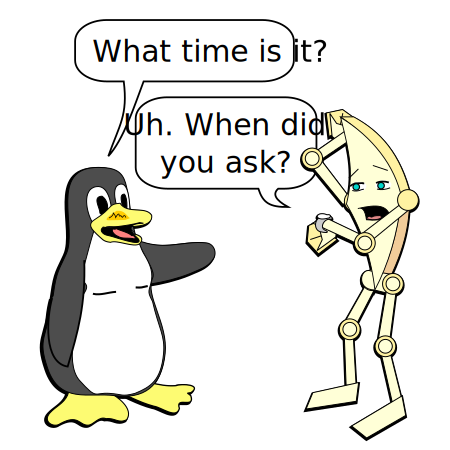
\includegraphics{cartoons/r-2014-What-time-is-it}}
\caption{What Time Is It?}
\ContributedBy{Figure}{fig:app:questions:What Time Is It?}{Melissa Broussard}
\end{figure}

멀티코어 컴퓨터 시스템에서의 시간 관리에서의 핵심적 문제가
\cref{fig:app:questions:What Time Is It?} 로 그려져 있습니다.
한가지 문제는 시간을 읽는데 시간이 걸린다는 겁니다.
어떤 명령은 하드웨어 시계를 읽을거고, 이 읽기 오퍼레이션을 완료하기 위해
off-core (더 나쁜 경우 off-socket) 으로 나가야 할수도 있습니다.
읽혀진 값에 대한 어떤 연산을 해야할 수도 있는데, 예를 들어 요구된 포맷으로
변환하기 위해, network time protocol (NTP) 조정을 위해, 등등이 있겠습니다.
그러니 결국 반환된 시간은 초래된 시간 간격의 시작, 끝, 또는 그 사이 어디에
맞춰져 있을까요?

더 나쁜게, 시간을 읽는 쓰레드는 인터럽트 당하거나 preemption 당할 수도
있습니다.
더 나아가, 시간을 읽는 시점과 그 시간의 실제 사용 사이에 어떤 연산이 있을
겁니다.
이 두개의 가능성 모두 이 불확정 시간을 늘립니다.

\iffalse

A key issue with timekeeping on multicore computer systems is illustrated
by \cref{fig:app:questions:What Time Is It?}.
One problem is that it takes time to read out the time.
An instruction might read from a hardware clock, and might
have to go off-core (or worse yet, off-socket) to complete
this read operation.
It might also be necessary to do some computation on the value read out,
for example, to convert it to the desired format, to apply network time
protocol (NTP) adjustments, and so on.
So does the time eventually returned correspond to the beginning of
the resulting time interval, the end, or somewhere in between?

Worse yet, the thread reading the time might be interrupted or preempted.
Furthermore, there will likely be some computation between reading out
the time and the actual use of the time that has been read out.
Both of these possibilities further extend the interval of uncertainty.

\fi

한가지 방법은 시간을 두번 읽고 타임스탬프가 만들어지는 이 오퍼레이션의 각 방향
중 하나에 있는, 이 두 읽기의 수치적 중간값을 사용하는 것입니다.
그럼 이 두 읽기 사이의 차이는 중간의 오퍼레이션이 수행된 시간의 불확정성의
측정값이 됩니다.

물론, 많은 경우 정확한 시간이 필요합니다.
예를 들어, 인간 사용자의 이익을 위한 시간을 출력하는 경우, 우린 내부의
하드웨어와 소프트웨어 지연이 쓸모없어지는 인간의 느린 반사속도에 기댈 수
있습니다.
비슷하게, 어떤 서버가 클라이언트로의 응답에 시간을 기록해야 한다면, 요청의
도착과 응답의 전송 사이 어느 시간이든 잘 동작할 겁니다.

\iffalse

One approach is to read the time twice, and take the arithmetic mean
of the two readings, perhaps one on each side of the operation being
timestamped.
The difference between the two readings is then a measure of uncertainty
of the time at which the intervening operation occurred.

Of course, in many cases, the exact time is not necessary.
For example, when printing the time for the benefit of a human user,
we can rely on slow human reflexes to render internal hardware and
software delays irrelevant.
Similarly, if a server needs to timestamp the response to a client, any
time between the reception of the request and the transmission of the
response will do equally well.

\fi

% @@@ Scheduling ticks

% @@@ Tickless operation

% @@@ Timers

% @@@ Current time, monotonic operation

% @@@ The many ways in which time can appear to go backwards

% @@@ Causality, the only real time in SMP (or distributed) systems

